\documentclass{article}
\usepackage[utf8]{inputenc}

\title{Github-Overleaf-Test}
\author{Mike Thielvoldt}
\date{October 2019}

\usepackage{natbib}
\usepackage{graphicx}

\begin{document}

\maketitle

\section{God is a prankster?}

Overleaf version 3 edit from remote

\begin{figure}[h!]
\centering
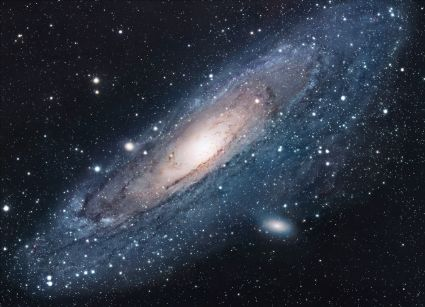
\includegraphics[scale=1.7]{universe}
\caption{A galaxy}
\label{fig:universe}
\end{figure}


\section{Thought-provoking Passages}
``I always thought something was fundamentally wrong with the universe'' \citep{adams1995hitchhiker}
\newline

``God does not play dice with the universe; He plays an ineffable game of His own devising, which might be compared, from the perspective of any of the other players [i.e. everybody], to being involved in an obscure and complex variant of poker in a pitch-dark room, with blank cards, for infinite stakes, with a Dealer who won't tell you the rules, and who smiles all the time.'' \citep{pratchett1990goodomens}

\bibliographystyle{plain}
\bibliography{references}
\end{document}
